From the given information, 
To find angle C:
\begin{align}
\angle{C} = \ang{70}
\end{align}
and 
\begin{align}
  a&= b\brak{\frac{\sin{A}}{\sin{B}}} 
\\
  &= 7.913611
  \end{align}
%  
Thus, the coordinates are 
\begin{align}
  \vec{C} =\myvec{0 \\ 0},
  \vec{B} =a\myvec{\cos{\ang{70}} \\ \sin{\ang{70}}},
  \vec{A} =\myvec{7 \\ 0}
  \end{align}
  
\begin{figure}[!h]
\centering
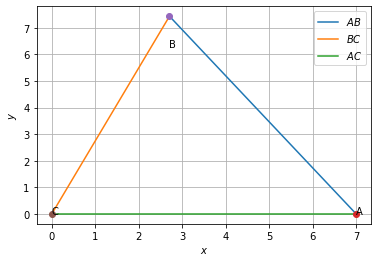
\includegraphics[width=\columnwidth]{solutions/july/2/4/Figure 1.jpeg}
\caption{$\triangle ABC$}
\label{fig:triangle}	
\end{figure}
To find side $a$
The vertices of $\triangle ABC$ are
Lines AB,BC,CA are then generated and plotted using these coordinates to construct $\triangle ABC$
Plot of the $\triangle ABC$:

\end{document}
